\chapter{Generalizzazione e validazione (introduzione)}\label{ch-04}

La quarta lezione conclude l'introduzione al ML affrontando il tema
centrale del corso: la \textbf{generalizzazione}. Attraverso un esempio
concreto (il fitting di polinomi) si vedono i fenomeni di
\textbf{underfitting} e \textbf{overfitting}, si dà una prima
formalizzazione con la \textbf{Statistical Learning Theory} e la
\textbf{VC-dimension}, e si introducono le tecniche di base di
\textbf{validazione}, le misure di accuratezza per la classificazione e
il ciclo di progettazione di un sistema di ML.

\section{Il ML in breve}\label{il-ml-in-breve}

Riepiloghiamo gli ingredienti visti nelle lezioni precedenti:

\begin{itemize}
\tightlist
\item
  \textbf{Dati}: l'esperienza disponibile, rappresentata come vettori,
  strutture, ecc.
\item
  \textbf{Task}: supervisionato (classificazione, regressione), non
  supervisionato, \ldots{} Ad esempio, dati esempi etichettati, trovare
  una buona approssimazione della \(f\) sconosciuta.
\item
  \textbf{Modello}: descrive le relazioni tra i dati e definisce la
  classe di funzioni che la macchina può implementare (lo spazio delle
  ipotesi).
\item
  \textbf{Algoritmo di apprendimento}: dati task e modello, esegue una
  ricerca (euristica) nello spazio delle ipotesi valide sui dati,
  adattando i parametri liberi del modello.
\item
  \textbf{Validazione}: valuta la capacità di generalizzazione
  dell'ipotesi trovata.
\end{itemize}

Il messaggio di fondo resta: \emph{facile usare strumenti di ML} contro
\emph{uso corretto e consapevole del ML}.

\section{I problemi fondamentali del
ML}\label{i-problemi-fondamentali-del-ml}

\subsection{Un problema mal posto}\label{un-problema-mal-posto}

Inferire funzioni generali da dati noti è un \textbf{problema mal
posto}: in linea di principio la soluzione non è unica, e con dati
finiti non possiamo aspettarci di trovare la soluzione esatta. Per
questo si lavora con uno \textbf{spazio delle ipotesi ristretto}
(ricordiamo il bias induttivo). Due domande guidano lo studio dei
modelli:

\begin{itemize}
\tightlist
\item
  \textbf{Cosa possiamo rappresentare?} (se una funzione non è
  rappresentabile, non può nemmeno essere appresa);
\item
  \textbf{Cosa possiamo apprendere?} (domanda secondaria rispetto alla
  prima).
\end{itemize}

\subsection{Generalizzazione e
overfitting}\label{generalizzazione-e-overfitting}

Distinguiamo la \textbf{fase di apprendimento}, in cui si costruisce il
modello (incluso il training), dalla \textbf{fase di predizione}, in cui
si valuta la funzione appresa su campioni nuovi (la capacità di
generalizzazione).

\begin{boxdefinition}{Ipotesi dell'apprendimento induttivo}

\emph{Qualsiasi ipotesi \(h\) che approssima bene \(f\) sugli esempi di
training approssimerà bene \(f\) anche su istanze nuove, mai viste.}

\end{boxdefinition}

Il punto interrogativo che il professore mette accanto a questa ipotesi
è voluto: \textbf{non è sempre vera}, ed è proprio qui che nasce
l'overfitting.

\begin{boxdefinition}{Overfitting}

Un learner fa \textbf{overfitting} sui dati se restituisce un'ipotesi
\(h \in H\) con errore vero (di generalizzazione, \emph{rischio}) \(R\)
ed errore empirico (di training) \(E\), quando esiste un'altra
\(h' \in H\) con \[
E' > E \qquad \text{ma} \qquad R' < R.
\] In altre parole, \(h'\) si adatta \emph{peggio} ai dati di training
ma è \emph{migliore} sui dati nuovi.

\end{boxdefinition}

L'aspetto critico diventa quindi la \textbf{stima dell'accuratezza}, che
si può affrontare in modo \textbf{teorico} (Statistical Learning Theory)
o \textbf{empirico} (errore su training e test, tecniche di
cross-validation).

\section{Un caso di studio: il fitting
polinomiale}\label{un-caso-di-studio-il-fitting-polinomiale}

Per vedere concretamente il ruolo della complessità del modello si usa
un esempio di regressione con un modello parametrico: lo spazio delle
ipotesi sono i \textbf{polinomi di grado \(M\)}, \[
h_\mathbf{w}(x) = w_0 + w_1 x + w_2 x^2 + \dots + w_M x^M = \sum_{j=0}^{M} w_j x^j.
\] La complessità dell'ipotesi cresce con il grado \(M\); \(l\) è il
numero di esempi.

\begin{boxwarning}{Esempio artificiale}

È un task semplificato e irrealistico: una sola variabile di input, e
conosciamo in anticipo la funzione target. Serve solo a visualizzare i
concetti.

\end{boxwarning}

La funzione target è \(\sin(2\pi x)\) a cui si aggiunge \textbf{rumore
gaussiano}: per questo i campioni non stanno esattamente sulla curva
verde ``vera''.

\begin{figure}[htbp]
\centering
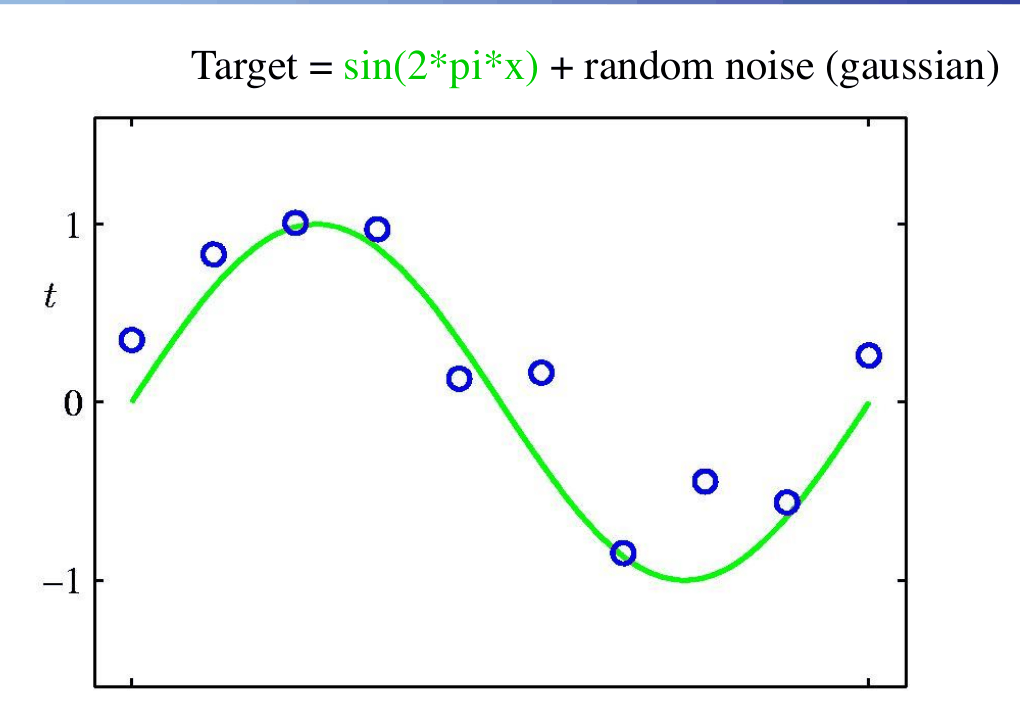
\includegraphics[width=0.54\linewidth,height=0.42\textheight,keepaspectratio]{images/04-l4_target-seno.png}
\caption{La funzione target \(\sin(2\pi x)\) (in verde) e i campioni rumorosi di
training (in blu).}
\end{figure}

Per trovare i parametri migliori si minimizza la \textbf{somma degli
errori quadratici}: \[
E(\mathbf{w}) = \sum_{p=1}^{l} \big(y_p - h_\mathbf{w}(x_p)\big)^2,
\] dove \(p\) indica l'esempio, \(y_p\) il suo target,
\(h_\mathbf{w}(x_p)\) l'uscita del modello nel punto \(x_p\) (qui \(x\)
è una sola variabile, \(n = 1\)).

\subsection{Effetto del grado del
polinomio}\label{effetto-del-grado-del-polinomio}

\begin{figure}[htbp]
\centering
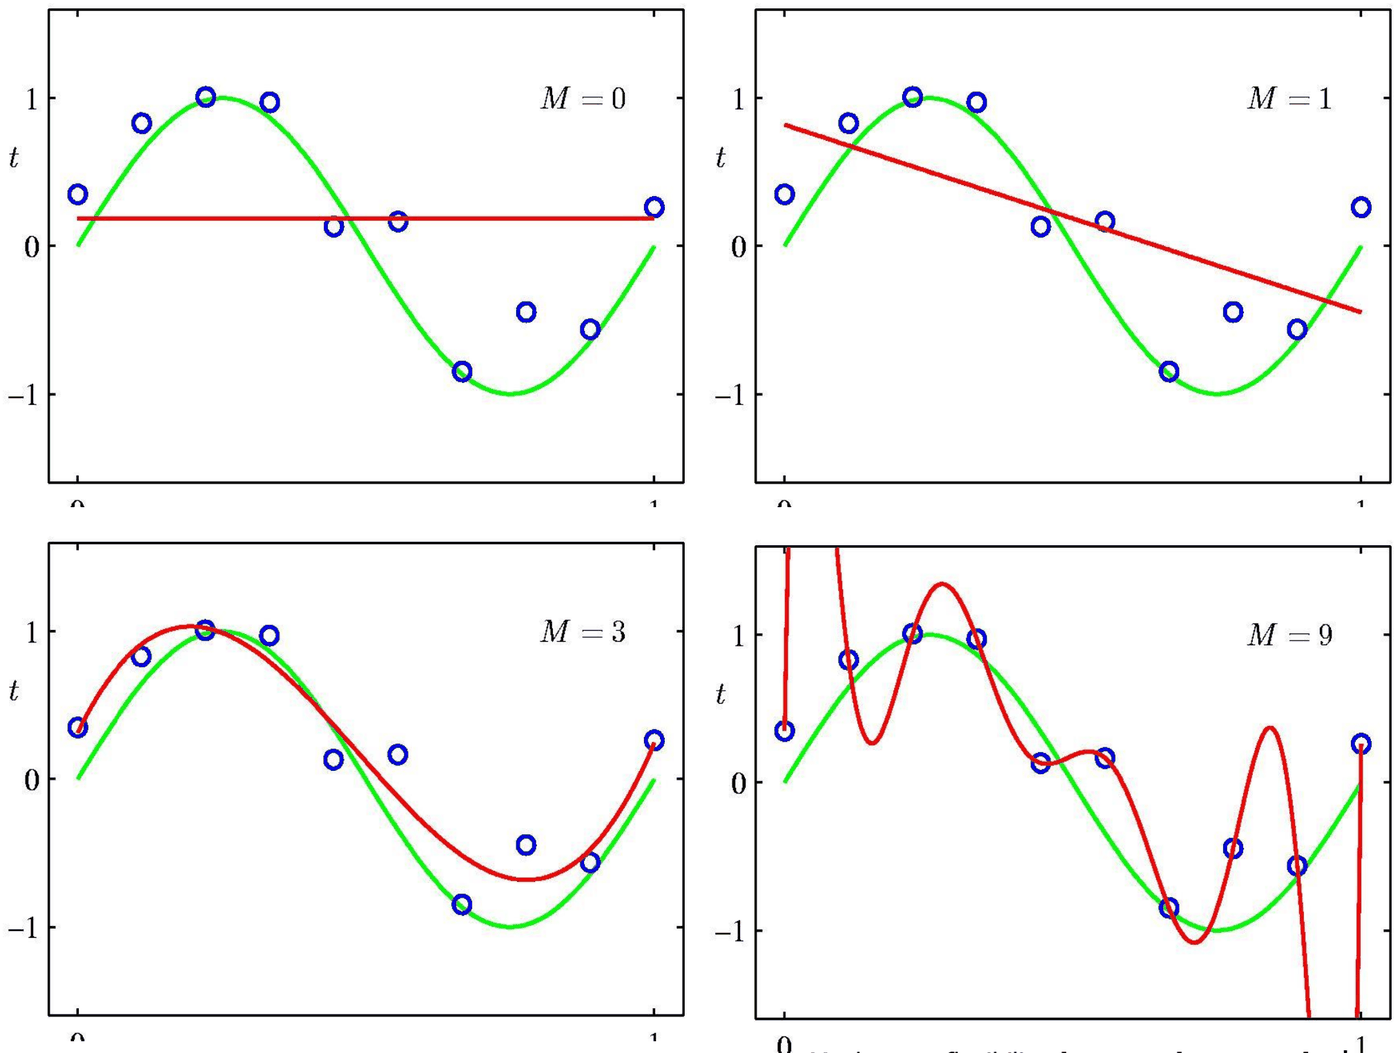
\includegraphics[width=0.91\linewidth,height=0.42\textheight,keepaspectratio]{images/04-l4_polinomi.png}
\caption{Fitting con polinomi di grado \(M = 0, 1, 3, 9\) (in rosso) rispetto
alla funzione vera (in verde).}
\end{figure}

\begin{itemize}
\tightlist
\item
  \textbf{\(M = 0\)} (costante) e \textbf{\(M = 1\)} (retta): il modello
  è \textbf{troppo semplice} rispetto alla funzione target e non riesce
  a coglierne l'andamento. È l'\textbf{underfitting}.
\item
  \textbf{\(M = 3\)}: più flessibilità è utile, e la curva approssima
  bene il seno.
\item
  \textbf{\(M = 9\)}: con 10 punti e 10 parametri il polinomio passa
  \textbf{esattamente} per tutti i dati: \(E(\mathbf{w}) = 0\) sul
  training! Ma la curva oscilla violentemente tra i punti e rappresenta
  malissimo la funzione vera: il modello è troppo complesso e
  \textbf{impara anche il rumore}. È l'\textbf{overfitting}. E l'errore
  sul test set?
\end{itemize}

\subsection{\texorpdfstring{Errore di training e di test al variare di
\(M\)}{Errore di training e di test al variare di M}}\label{errore-di-training-e-di-test-al-variare-di-m}

Per confrontare i modelli si usa il \textbf{Root-Mean-Square error},
\(E_{RMS} = \sqrt{2E(\mathbf{w}^*)/l}\), dove \(E(\mathbf{w}^*)\) è
l'errore del modello addestrato. La divisione per \(l\) permette di
confrontare dataset di dimensione diversa, e la radice riporta l'errore
sulla stessa scala del target.

\begin{figure}[htbp]
\centering
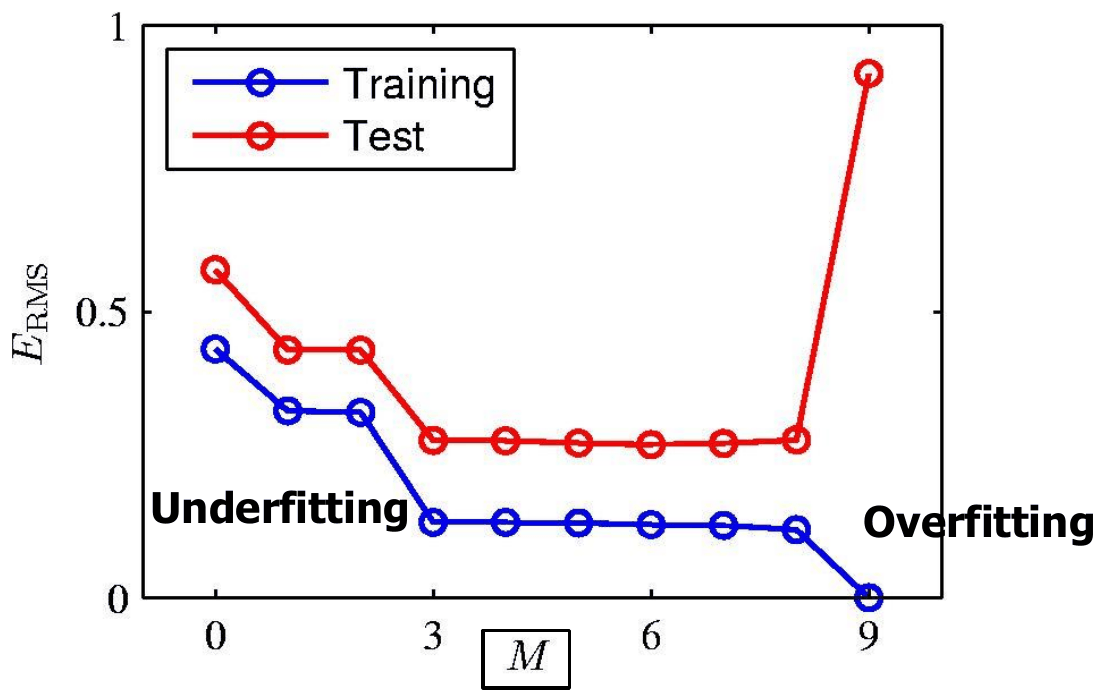
\includegraphics[width=0.60\linewidth,height=0.42\textheight,keepaspectratio]{images/04-l4_rms-vs-M.png}
\caption{Errore RMS di training e di test al variare del grado \(M\): zona di
underfitting a sinistra, di overfitting a destra.}
\end{figure}

L'errore di training \textbf{decresce sempre} all'aumentare di \(M\),
perché un modello più flessibile può adattarsi meglio ai dati. L'errore
di test invece prima decresce, poi resta stabile e infine
\textbf{esplode} per \(M = 9\): è la firma dell'overfitting.

Anche i \textbf{coefficienti} ottimi \(\mathbf{w}^*\) sono rivelatori:

{\def\LTcaptype{none} % do not increment counter
\begin{longtable}[]{@{}lllll@{}}
\toprule\noalign{}
& \(M=0\) & \(M=1\) & \(M=3\) & \(M=9\) \\
\midrule\noalign{}
\endhead
\bottomrule\noalign{}
\endlastfoot
\(w_0^*\) & 0,19 & 0,82 & 0,31 & 0,35 \\
\(w_1^*\) & & −1,27 & 7,99 & 232,37 \\
\(w_2^*\) & & & −25,43 & −5321,83 \\
\(w_3^*\) & & & 17,37 & 48568,31 \\
\(w_4^*\) & & & & −231639,30 \\
\(w_5^*\) & & & & 640042,26 \\
\(w_6^*\) & & & & −1061800,52 \\
\(w_7^*\) & & & & 1042400,18 \\
\(w_8^*\) & & & & −557682,99 \\
\(w_9^*\) & & & & 125201,43 \\
\end{longtable}
}

\begin{boxtip}{Pesi enormi = overfitting}

Nel polinomio di grado 9 i coefficienti diventano \textbf{enormi} e di
segno alterno: si compensano a vicenda per far passare la curva
esattamente per ogni punto, producendo oscillazioni fortissime. Questa
osservazione è alla base della \textbf{regolarizzazione} (che vedremo
con i modelli lineari e le reti neurali): penalizzare pesi grandi è un
modo per controllare la complessità.

\end{boxtip}

\subsection{Effetto della quantità di
dati}\label{effetto-della-quantituxe0-di-dati}

Cosa succede se, a parità di modello (\(M = 9\)), aumentiamo i dati?

\begin{figure}[htbp]
\centering
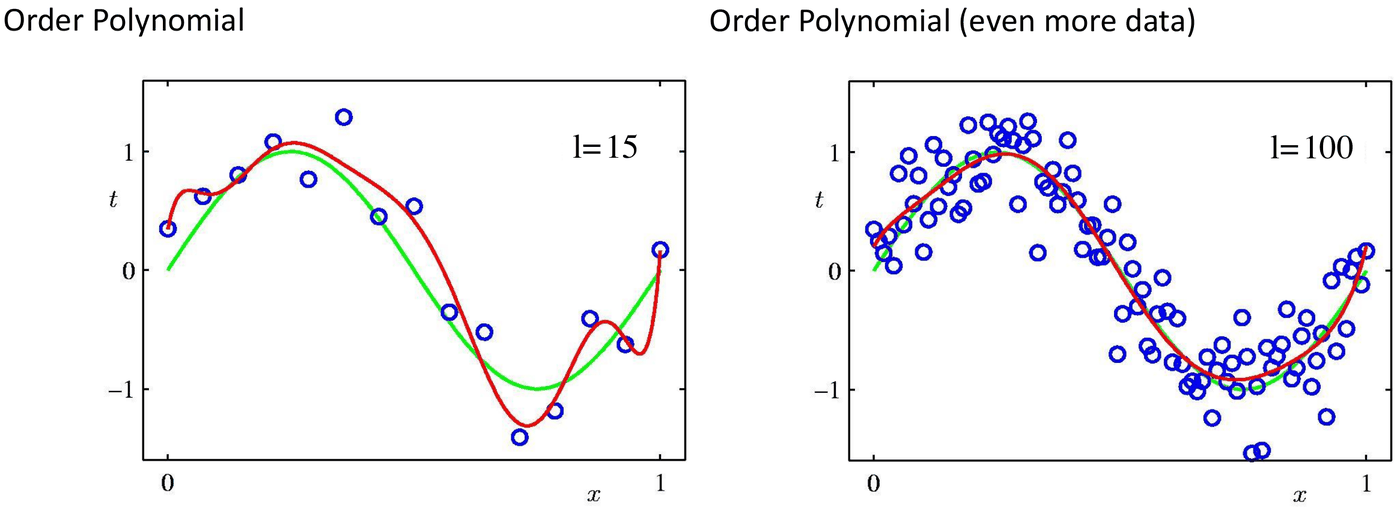
\includegraphics[width=0.91\linewidth,height=0.42\textheight,keepaspectratio]{images/04-l4_polinomio9-dati.png}
\caption{Polinomio di grado 9 con \(l = 15\) e \(l = 100\) esempi: con più dati
l'overfitting si riduce.}
\end{figure}

Con 15 esempi il polinomio di grado 9 oscilla ancora, ma molto meno; con
100 esempi segue quasi perfettamente il seno. \textbf{Con più dati si
possono usare modelli più complessi} senza cadere nell'overfitting.

\begin{boxabstract}{Cosa abbiamo imparato}

La capacità di generalizzazione (misurata come rischio o errore di test)
va studiata in relazione a: - l'\textbf{errore di training} e le zone di
underfitting e overfitting; - la \textbf{complessità del modello}; - il
\textbf{numero di dati}.

La \textbf{Statistical Learning Theory} è la teoria generale che lega
questi tre elementi.

\end{boxabstract}

\section{Verso la Statistical Learning
Theory}\label{verso-la-statistical-learning-theory}

\subsection{Il setting formale
(semplificato)}\label{il-setting-formale-semplificato}

Vogliamo approssimare una funzione sconosciuta \(f(\mathbf{x})\), dove
il target è \(d = f(\mathbf{x}) + \text{rumore}\).

Idealmente vorremmo minimizzare la \textbf{funzione di rischio} (errore
vero), calcolata su \textbf{tutti} i dati possibili: \[
R = \int L\big(d, h(\mathbf{x})\big)\, dP(\mathbf{x}, d),
\] dove \(P(\mathbf{x}, d)\) è la distribuzione di probabilità
(sconosciuta) dei dati e \(L\) è una loss, ad esempio
\(L(h(\mathbf{x}), d) = (d - h(\mathbf{x}))^2\). Si cerca quindi
\(h \in H\) che minimizzi \(R\).

Ma abbiamo solo un dataset finito
\(TR = \{(\mathbf{x}_p, d_p)\}_{p=1}^{l}\). Allora si minimizza il
\textbf{rischio empirico} (errore di training), trovando i valori
migliori dei parametri liberi: \[
R_{emp}(h, TR) = \frac{1}{l} \sum_{p=1}^{l} \big(d_p - h(\mathbf{x}_p)\big)^2.
\] Questo è il principio induttivo di \textbf{Empirical Risk
Minimization} (ERM). La domanda cruciale è: \textbf{possiamo usare
\(R_{emp}\) per approssimare \(R\)?}

\begin{figure}[htbp]
\centering
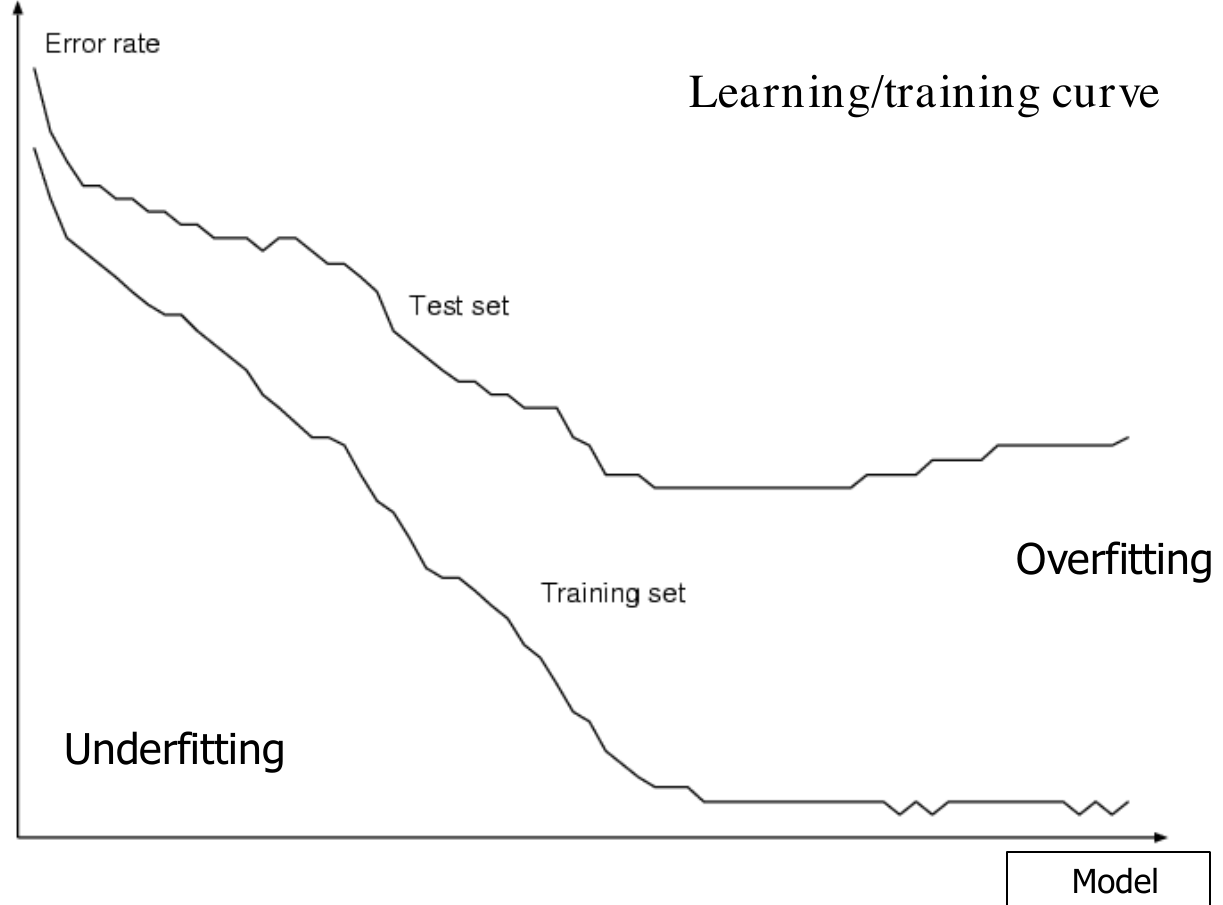
\includegraphics[width=0.57\linewidth,height=0.42\textheight,keepaspectratio]{images/04-l4_curva-apprendimento.png}
\caption{Comportamento tipico dell'apprendimento al crescere della complessità
del modello.}
\end{figure}

\subsection{VC-dimension e bound sul
rischio}\label{vc-dimension-e-bound-sul-rischio}

La \textbf{VC-dimension} (Vapnik-Chervonenkis) è una misura della
\textbf{complessità} di \(H\), cioè della sua flessibilità
nell'adattarsi ai dati (per modelli lineari o polinomi è legata al
numero di parametri; sarà definita formalmente più avanti).

\begin{boxtheorem}{VC-bound}

Con probabilità \(1 - \delta\) vale: \[
\underbrace{R}_{\text{rischio garantito}} \;\le\; R_{emp} + \underbrace{\varepsilon\left(\frac{1}{l}, VC, \frac{1}{\delta}\right)}_{\text{VC-confidence}}
\] dove la \textbf{VC-confidence} \(\varepsilon\) è una funzione che
\textbf{cresce con la VC-dimension} e \textbf{decresce con il numero di
dati \(l\)} (e con \(\delta\)).

\end{boxtheorem}

Il parametro \(\delta\) è la \textbf{confidenza}: regola la probabilità
che il bound valga (ad esempio \(\delta = 0{,}01\) significa che il
bound vale con probabilità \(0{,}99\)).

Questo bound \textbf{spiega} underfitting e overfitting:

\begin{itemize}
\tightlist
\item
  \textbf{più dati} (\(l\) alto) → VC-confidence più bassa, e il bound
  si avvicina a \(R\): il rischio empirico diventa una buona stima di
  quello vero;
\item
  \textbf{modello troppo semplice} (VC-dim bassa) → \(\varepsilon\)
  piccolo, ma \(R_{emp}\) alto: \textbf{underfitting};
\item
  \textbf{modello troppo complesso} (VC-dim alta, \(l\) fissato) →
  \(R_{emp}\) basso, ma \(\varepsilon\) cresce, e con esso il bound su
  \(R\): \textbf{overfitting}.
\end{itemize}

\begin{figure}[htbp]
\centering
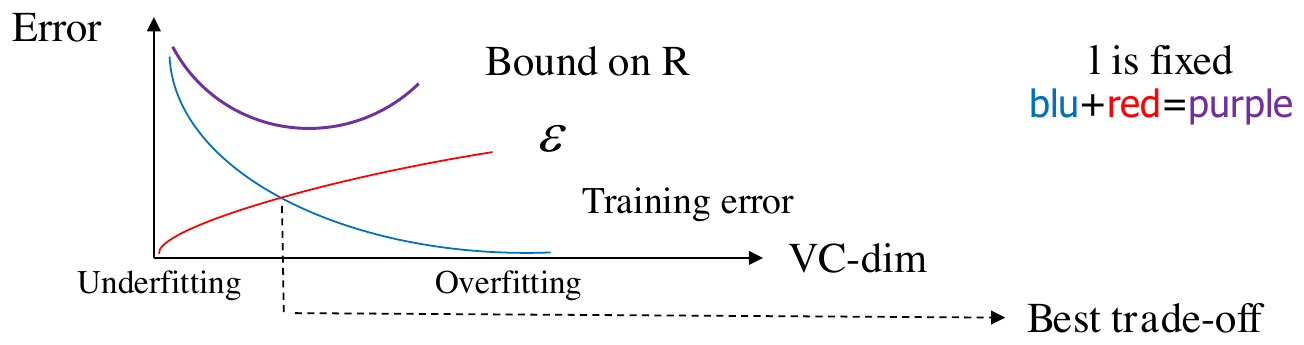
\includegraphics[width=0.80\linewidth,height=0.42\textheight,keepaspectratio]{images/04-l4_bound-vc.png}
\caption{Structural Risk Minimization: il bound su \(R\) (viola) è la somma
dell'errore di training (blu) e della VC-confidence (rossa); il suo
minimo è il miglior compromesso.}
\end{figure}

\begin{boxdefinition}{Structural Risk Minimization (SRM)}

Invece di minimizzare solo \(R_{emp}\), si \textbf{minimizza il bound},
cioè la somma di errore di training e VC-confidence. Questo formalizza
il concetto di \textbf{controllo della complessità del modello}: un
compromesso tra complessità (VC-dim) e accuratezza sul training
(fitting).

\end{boxdefinition}

Un esempio concreto di bound è \[
R \le R_{emp} + \varepsilon\left(\frac{VC}{l}, -\frac{\ln\delta}{l}\right),
\] e ne esistono diverse formulazioni per diverse classi di funzioni e
task. In parole semplici: \textbf{si può approssimare bene \(f\) dagli
esempi purché si abbia un buon numero di dati e la complessità del
modello sia adatta al problema}. Bisogna adattarsi ai dati il più
possibile per evitare l'underfitting (alto \(R_{emp}\)), ma non troppo,
per evitare l'overfitting (dovuto alla crescita della VC-confidence).

\begin{boxnote}{Oltre il compromesso classico}

Fenomeni più recenti come la \textbf{double descent}, la
sovra-parametrizzazione e il \emph{benign overfitting} (tipici delle
reti profonde) sembrano sfidare questa visione e verranno discussi più
avanti nel corso.

\end{boxnote}

\subsection{Perché la SLT è
importante}\label{perchuxe9-la-slt-uxe8-importante}

La SLT permette di inquadrare formalmente il problema della
generalizzazione e dell'overfitting, fornendo \textbf{upper bound
analitici} al rischio \(R\) indipendentemente dal tipo di algoritmo o
dai dettagli del modello. Mostra che il ML è \textbf{ben fondato}: il
rischio si può limitare analiticamente, e pochi concetti sono
fondamentali. Ha inoltre portato a nuovi modelli (le \textbf{SVM}) che
considerano direttamente il controllo della complessità, e spiega la
differenza principale tra il ML e i metodi di ottimizzazione puri (che
forniscono le tecniche per fare \emph{fitting}): nel ML l'obiettivo non
è minimizzare l'errore sui dati, ma sui dati \emph{futuri}.

Restano aperte domande pratiche: come misurare la complessità? Come
trovare il miglior compromesso tra fitting e complessità?

\begin{boxquestion}{Esercizi proposti dal professore}

\begin{itemize}
\tightlist
\item
  Perché un errore di training nullo non implica necessariamente una
  buona soluzione?
\item
  Collegare underfitting e overfitting all'interpretazione della
  disuguaglianza della SLT e all'esempio dei polinomi.
\item
  Guardando la definizione di overfitting, individuare \(h\) e \(h'\)
  sul grafico del bound SLT. \emph{(Suggerimento: \(h\) sta a destra del
  minimo, con \(R_{emp}\) più basso ma bound più alto; \(h'\) sta vicino
  al minimo.)}
\item
  Il rumore è la causa dell'overfitting, o lo è il compromesso di
  complessità? Si può avere overfitting anche con dati perfettamente
  puliti? \emph{(Sì: anche senza rumore, un polinomio di grado molto
  alto interpolando pochi punti di una funzione liscia può oscillare
  molto tra un punto e l'altro; il problema è la complessità eccessiva
  rispetto ai dati disponibili.)}
\end{itemize}

\end{boxquestion}

\section{Validazione}\label{validazione}

La valutazione delle prestazioni di un sistema di ML è la valutazione
della sua \textbf{accuratezza predittiva}. Attenzione: \textbf{le
prestazioni sui dati di training danno una valutazione troppo
ottimistica}. Da qui il mantra ``validazione, validazione,
validazione''. Qui si dà un'introduzione; la validazione sarà ripresa in
lezioni dedicate.

\subsection{I due obiettivi della
validazione}\label{i-due-obiettivi-della-validazione}

\begin{boxdefinition}{Model selection e model assessment}

\begin{itemize}
\tightlist
\item
  \textbf{Model selection}: stimare le prestazioni (errore di
  generalizzazione) di \textbf{diversi modelli} per scegliere il
  migliore. Include la ricerca dei migliori \textbf{iperparametri} (es.
  il grado del polinomio). \emph{Restituisce un modello.}
\item
  \textbf{Model assessment}: scelto il modello finale, stimarne l'errore
  di predizione (rischio) su \textbf{nuovi dati di test}, come misura
  della qualità del modello scelto. \emph{Restituisce una stima.}
\end{itemize}

\end{boxdefinition}

\begin{boxwarning}{Regola d'oro}

Tenere \textbf{separati gli obiettivi} e usare \textbf{insiemi di dati
separati} per ciascuno. Se il test set viene usato per scegliere il
modello, la stima finale non è più affidabile (è ottimistica).

\end{boxwarning}

Nel mondo ideale avremmo un grande training set (per trovare l'ipotesi
migliore), un grande validation set per la model selection e un test set
esterno molto grande. Con dataset finiti, spesso piccoli, si può solo
\textbf{stimare} la generalizzazione.

\subsection{Hold-out}\label{hold-out}

Nella tecnica di base, \textbf{hold-out}, il dataset \(D\) viene
partizionato in tre insiemi \textbf{disgiunti}:

\begin{itemize}
\tightlist
\item
  \textbf{Training set (TR)}: usato per eseguire l'algoritmo di
  apprendimento;
\item
  \textbf{Validation set (VL)} o \emph{selection set}: usato per
  scegliere il modello migliore (es. tuning degli iperparametri);
\item
  \textbf{Test set (TS)}: usato \textbf{solo} per la model assessment,
  mai per scegliere o regolare \(h\).
\end{itemize}

TR e VL insieme formano il \textbf{development/design set}; il test set
(ad esempio il 25--30\% dei dati) viene tenuto da parte.

\begin{figure}[htbp]
\centering
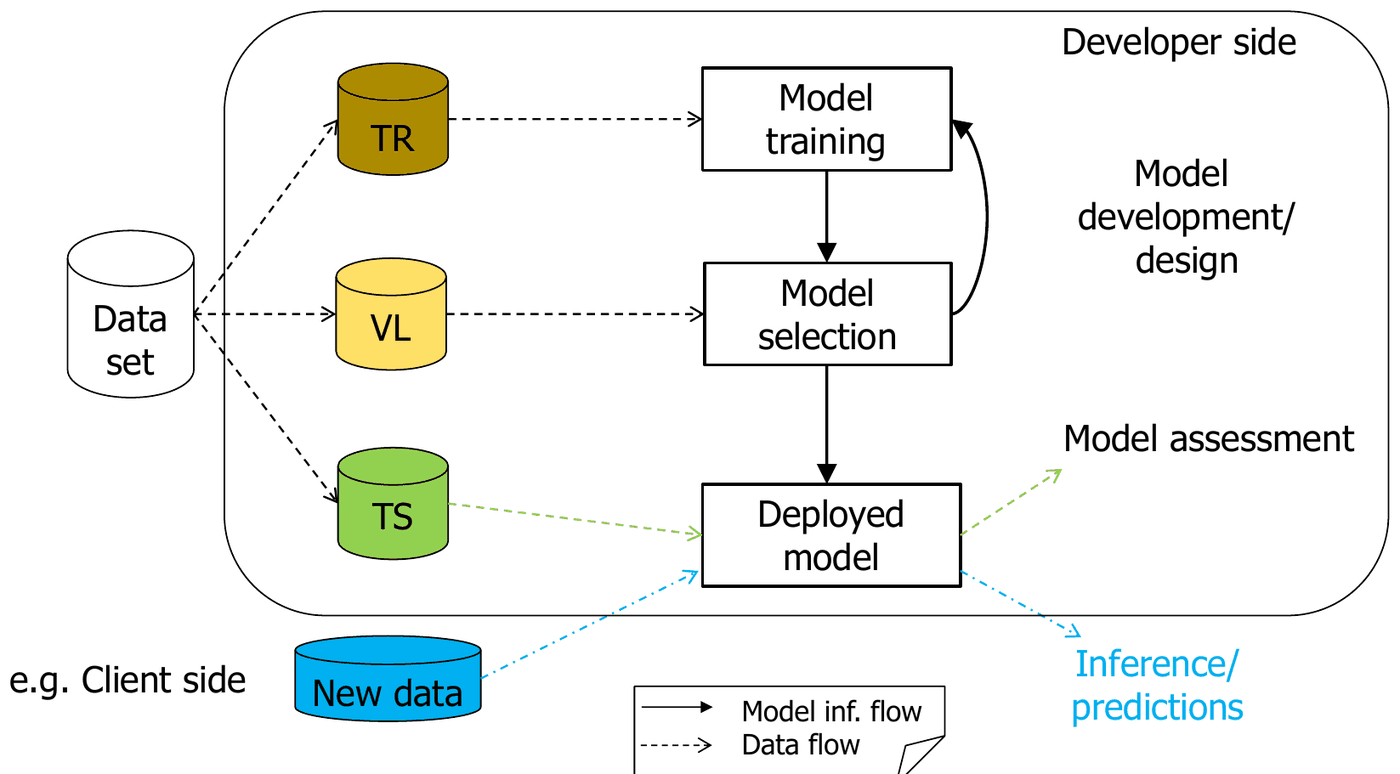
\includegraphics[width=0.86\linewidth,height=0.42\textheight,keepaspectratio]{images/04-l4_schema-tr-vl-ts.png}
\caption{Ruolo di TR, VL e TS: sviluppo del modello lato sviluppatore, uso in
inferenza lato cliente.}
\end{figure}

\subsection{K-fold cross-validation
(anticipazione)}\label{k-fold-cross-validation-anticipazione}

L'hold-out può sfruttare male i dati, soprattutto se sono pochi. Nella
\textbf{K-fold cross-validation}:

\begin{enumerate}
\def\labelenumi{\arabic{enumi}.}
\tightlist
\item
  si divide \(D\) in \(k\) sottoinsiemi mutuamente esclusivi
  \(D_1, \dots, D_k\);
\item
  per ogni \(i\) si addestra su \(D \setminus D_i\) e si valuta su
  \(D_i\);
\item
  si combinano i \(k\) risultati.
\end{enumerate}

\begin{figure}[htbp]
\centering
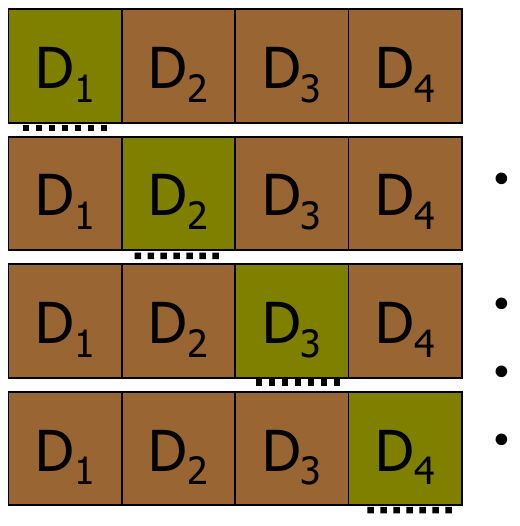
\includegraphics[width=0.29\linewidth,height=0.42\textheight,keepaspectratio]{images/04-l4_kfold.png}
\caption{4-fold cross-validation: a turno ogni fold fa da insieme di validazione.}
\end{figure}

Così tutti i dati vengono usati sia per l'addestramento sia per la
validazione (o il test). Si può applicare sia per lo split di
validazione sia per quello di test. Le questioni aperte sono quante fold
usare (3, 5, 10, fino a \emph{leave-one-out}), il costo computazionale
spesso elevato e la combinazione con altri schemi (validation set,
doppia K-fold). Sarà ripresa in dettaglio più avanti.

\section{Accuratezza nella
classificazione}\label{accuratezza-nella-classificazione}

\subsection{Matrice di confusione}\label{matrice-di-confusione}

Per un classificatore binario si confrontano classe reale e classe
predetta:

{\def\LTcaptype{none} % do not increment counter
\begin{longtable}[]{@{}lll@{}}
\toprule\noalign{}
Reale ~Predetto & Positivo & Negativo \\
\midrule\noalign{}
\endhead
\bottomrule\noalign{}
\endlastfoot
\textbf{Positivo} & TP (veri positivi) & FN (falsi negativi) \\
\textbf{Negativo} & FP (falsi positivi) & TN (veri negativi) \\
\end{longtable}
}

Da cui:

\begin{itemize}
\tightlist
\item
  \textbf{Accuratezza} \(= \dfrac{TP + TN}{\text{totale}}\): percentuale
  di pattern classificati correttamente;
\item
  \textbf{Sensibilità} (\emph{True Positive rate}, \emph{Recall})
  \(= \dfrac{TP}{TP + FN}\): quanti positivi veri vengono riconosciuti;
\item
  \textbf{Specificità} (\emph{True Negative rate})
  \(= \dfrac{TN}{FP + TN} = 1 - FPR\): quanti negativi veri vengono
  riconosciuti;
\item
  \textbf{Precisione} \(= \dfrac{TP}{TP + FP}\): quanti dei predetti
  positivi sono davvero positivi.
\end{itemize}

Un falso positivo equivale a un \textbf{falso allarme}.

\begin{boxwarning}{Attenzione all'accuratezza}

\begin{itemize}
\tightlist
\item
  Per la classificazione binaria, un'accuratezza del 50\% è quella di un
  predittore \textbf{casuale} (lancio di una moneta).
\item
  Con \textbf{dati sbilanciati} (es. 99\% di positivi) esiste un
  classificatore banale che risponde sempre ``positivo'' e ha il 99\% di
  accuratezza senza aver imparato nulla. In questi casi l'accuratezza da
  sola è fuorviante.
\end{itemize}

\end{boxwarning}

\subsection{Curva ROC}\label{curva-roc}

La \textbf{curva ROC} mostra il \emph{True Positive rate} (sensibilità)
in funzione del \emph{False Positive rate} (\(1 -\) specificità) al
variare della soglia di decisione del classificatore.

\begin{figure}[htbp]
\centering
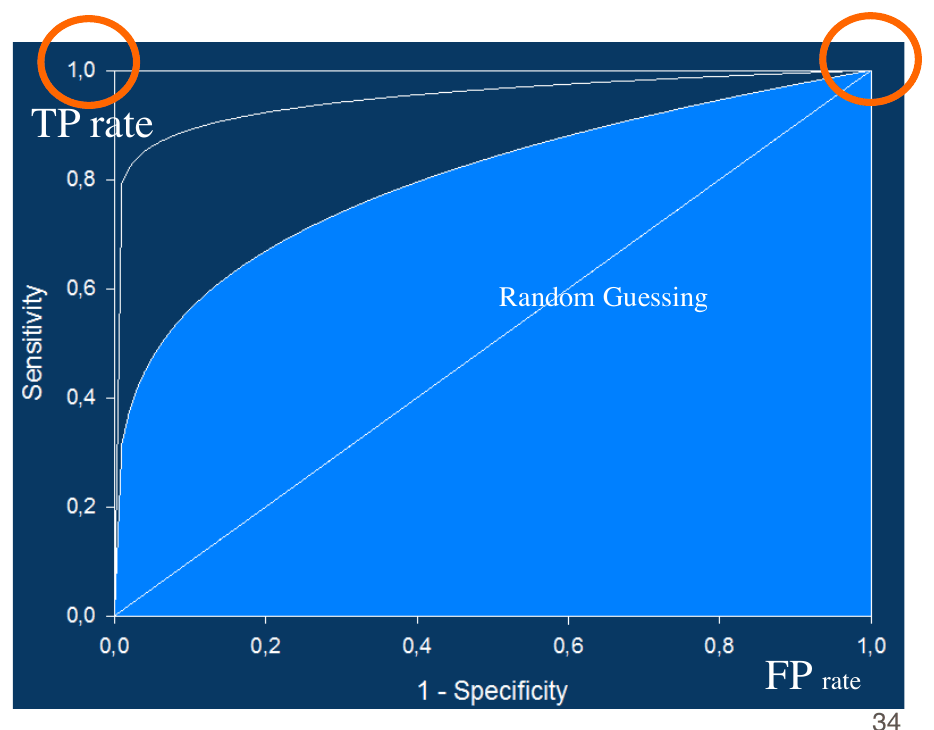
\includegraphics[width=0.49\linewidth,height=0.42\textheight,keepaspectratio]{images/04-l4_roc.png}
\caption{Curva ROC: la diagonale corrisponde al classificatore casuale; curve
migliori hanno un'area sottesa (AUC) maggiore.}
\end{figure}

La \textbf{diagonale} corrisponde al classificatore peggiore (casuale).
Le curve migliori salgono rapidamente verso l'angolo in alto a sinistra
(TPR alto con FPR basso) e hanno un'\textbf{AUC} (\emph{Area Under the
Curve}) più alta: il classificatore ideale ha AUC \(= 1\), quello
casuale \(0{,}5\).

\section{Il ciclo di progettazione}\label{il-ciclo-di-progettazione}

\begin{figure}[htbp]
\centering
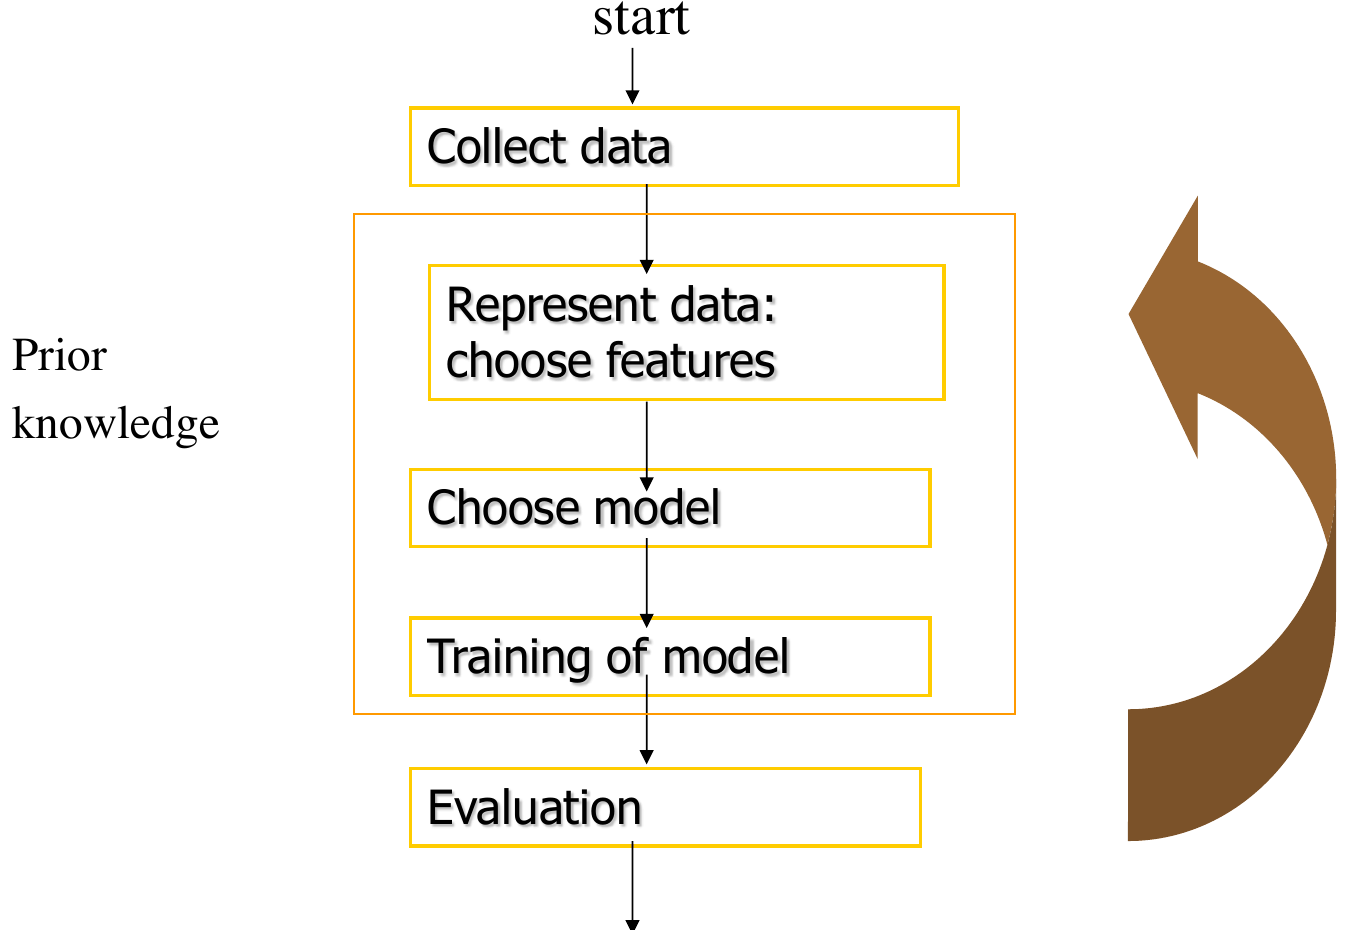
\includegraphics[width=0.57\linewidth,height=0.42\textheight,keepaspectratio]{images/04-l4_ciclo-progettazione.png}
\caption{Il ciclo di progettazione di un sistema di ML: un processo iterativo
guidato dalla conoscenza a priori.}
\end{figure}

\begin{enumerate}
\def\labelenumi{\arabic{enumi}.}
\tightlist
\item
  \textbf{Raccolta dei dati}: selezione, integrazione, pulizia. Serve un
  insieme di esempi abbastanza \textbf{grande e rappresentativo} per
  training e test.
\item
  \textbf{Rappresentazione dei dati}: dipende dal dominio e sfrutta la
  conoscenza a priori dell'esperto; comprende feature selection,
  rilevamento degli outlier, scalatura delle variabili, gestione dei
  dati mancanti. \textbf{Spesso è la fase più critica} per il successo
  complessivo.
\item
  \textbf{Scelta del modello}: formulazione del problema e delle
  ipotesi. Bisogna conoscere i \textbf{limiti di applicabilità} del
  modello e controllarne la complessità.
\item
  \textbf{Costruzione del modello} (il cuore del ML): tramite
  l'algoritmo di apprendimento sui dati di training.
\item
  \textbf{Valutazione}: la prestazione è l'\textbf{accuratezza
  predittiva}; si aggiungono l'interpretazione dei risultati, la
  spiegazione dei dati e l'estrazione di conoscenza.
\item
  \textbf{Deployment}.
\end{enumerate}

Il ciclo è iterativo: i risultati della valutazione possono richiedere
di tornare alle fasi precedenti.

\section{Errori di interpretazione}\label{errori-di-interpretazione}

Per ogni modello statistico (inclusi Data Mining e ML):

\begin{itemize}
\tightlist
\item
  si assume (spesso) una \textbf{causalità} e serve un insieme di dati
  \textbf{rappresentativo} del fenomeno. Il ML non funziona con
  variabili scorrelate o fenomeni casuali (lotterie); input non
  informativi portano a modelli e risultati scadenti;
\item
  \textbf{la causalità non si può inferire dalla sola analisi dei dati}:
  in Florida le persone sono in media più anziane che negli altri stati
  USA, ma non è il clima a farle vivere più a lungo (ci si trasferisce
  lì da pensionati). La dipendenza statistica può avere ragioni esterne
  ai dati.
\end{itemize}

Specifico per il ML: \textbf{modelli potenti aumentano il rischio},
perché si adattano anche a dati ``spazzatura''; e risultati \textbf{non
validati bene} possono portare a predizioni e interpretazioni
fuorvianti.

\begin{boxabstract}{Sintesi}

La generalizzazione dipende dal compromesso tra \textbf{complessità del
modello} e \textbf{quantità di dati}. Modelli troppo semplici fanno
\textbf{underfitting}, troppo complessi fanno \textbf{overfitting}
(errore di training basso, di test alto). La SLT formalizza tutto con il
\textbf{VC-bound} \(R \le R_{emp} + \varepsilon(1/l, VC, 1/\delta)\) e
suggerisce la \textbf{Structural Risk Minimization}. In pratica la
generalizzazione si stima con la \textbf{validazione}: \emph{model
selection} (su VL) e \emph{model assessment} (su TS), sempre su dati
separati.

\end{boxabstract}

\begin{boxquestion}{Possibili domande d'esame}

\begin{itemize}
\tightlist
\item
  Definire formalmente l'overfitting.
\item
  Descrivere l'esempio del fitting polinomiale: cosa succede al variare
  di \(M\) e di \(l\)?
\item
  Scrivere il VC-bound e spiegare come giustifica underfitting e
  overfitting.
\item
  Differenza tra rischio \(R\) e rischio empirico \(R_{emp}\); cos'è il
  principio ERM?
\item
  Differenza tra model selection e model assessment; perché servono
  insiemi separati?
\item
  Definire accuratezza, sensibilità, specificità, precisione; cos'è la
  curva ROC?
\end{itemize}

\end{boxquestion}
